\section{Experiment 1.1}

The next step was to gather more extensive data about the USB
transmissions, in order to narrow down the problems in experiment 1.
For this experiment, two different \acrshort{gpio} pins where used to
flag for two different states. The first one was set to toggle each
time the device triggered a general USB interrupt. When this interrupt
occurred, the device parsed the USB request and checked if it
contained a buffer with audio samples. If this was the case, it
toggled the second pin.

In order to measure the size of the data packets sent from the host
during each transmission, a USART output was included in the mocked
device program. Each time the device receives an interrupt containing
audio data, it measures the length of this data packet, and write it
to the UART output. This was then captured by the logic analyzer, and
parsed along with the rest of the measured data with the python
parser.

\todo{Explain USART}

For the UART to have time to write the length of each packet before
the next one arrived, it would need to output at a rate much higher
then the rate of USB messages. Experiment 1 showed that the rate of
the USB data transmitted from the host machine was around once every
two milliseconds, which results in 500 transmissions each second.
Using a sufficiently high UART rate, in this case 115200 bits/s, it
could be ensured that the UART would be able to output a sufficiently
large amount of bytes between each interrupt. 

\todo{Rewrite this so it makes sense}

Adding these extra signals resulting in the measurement in figure
\ref{fig:experiment-1-1-raw}. The outliers still remains, as can be
seen in the large pulse in the middle. But now it can be observed that
each of the interrupts seems to correspond to a valid audio packet, as
the rate of both pins are about the same. 

\begin{figure}[h]
	\caption{A piece of the captured data for experiment 1.1, in Saleaes
	analyzer software Logic.}
	\centering
	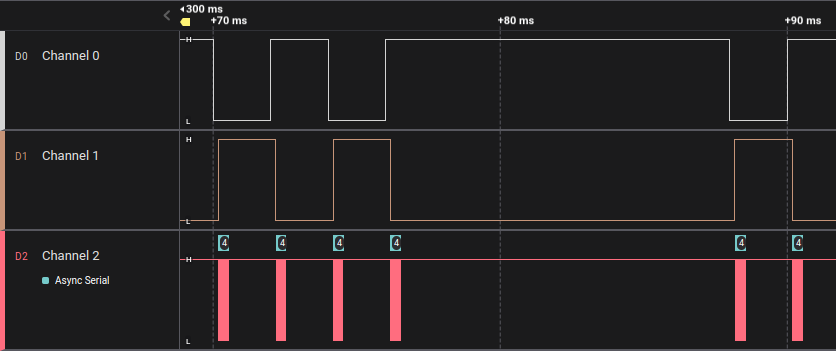
\includegraphics[width=0.8\textwidth]{Experiment-1/Experiment-1-1-raw.png}
	\label{fig:experiment-1-1-raw}
\end{figure}

The third reading is the serial output from the device. The large
headroom between the end of these transmissions to the next interrupt
indicates that the rate for the USART is high enough to not cause any
problems regarding timing. In figure \ref{fig:experiment-1-1-serial},
the message containing the length of a USB requests audio buffer is
shown to be 288 bytes long.

\begin{figure}[h]
	\caption{A zoomed in piece of the captured data for experiment
	1.1, showing the USART message being sent.}
	\centering
	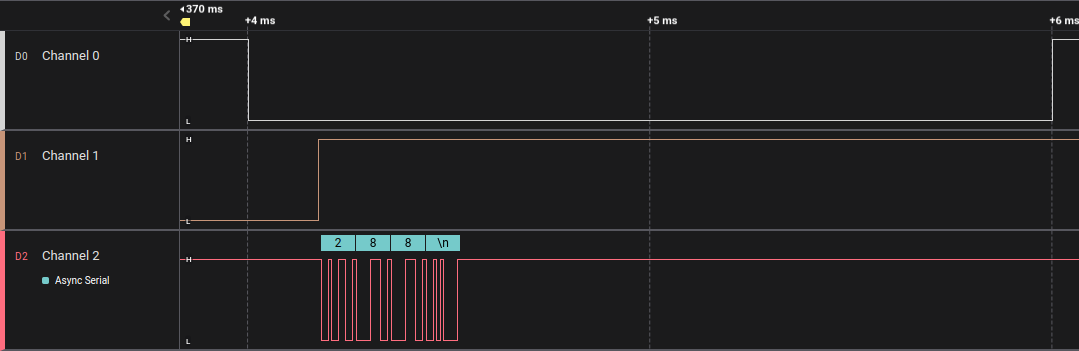
\includegraphics[width=0.8\textwidth]{Experiment-1/Experiment-1-1-serial.png}
	\label{fig:experiment-1-1-serial}
\end{figure}

Using the python parser resulted in the diagrams shown in figure
\ref{fig:experiment-1-1}. Here the outliers can still be observed. But
along with the interrupt rate, the length of the USB requests audio
buffer is shown to be at a steady length of 288 bytes/message.

\begin{figure}[h]
	\caption{Rate over time and buffer length over time respectively
	for experiment 1.1}
	\centering
	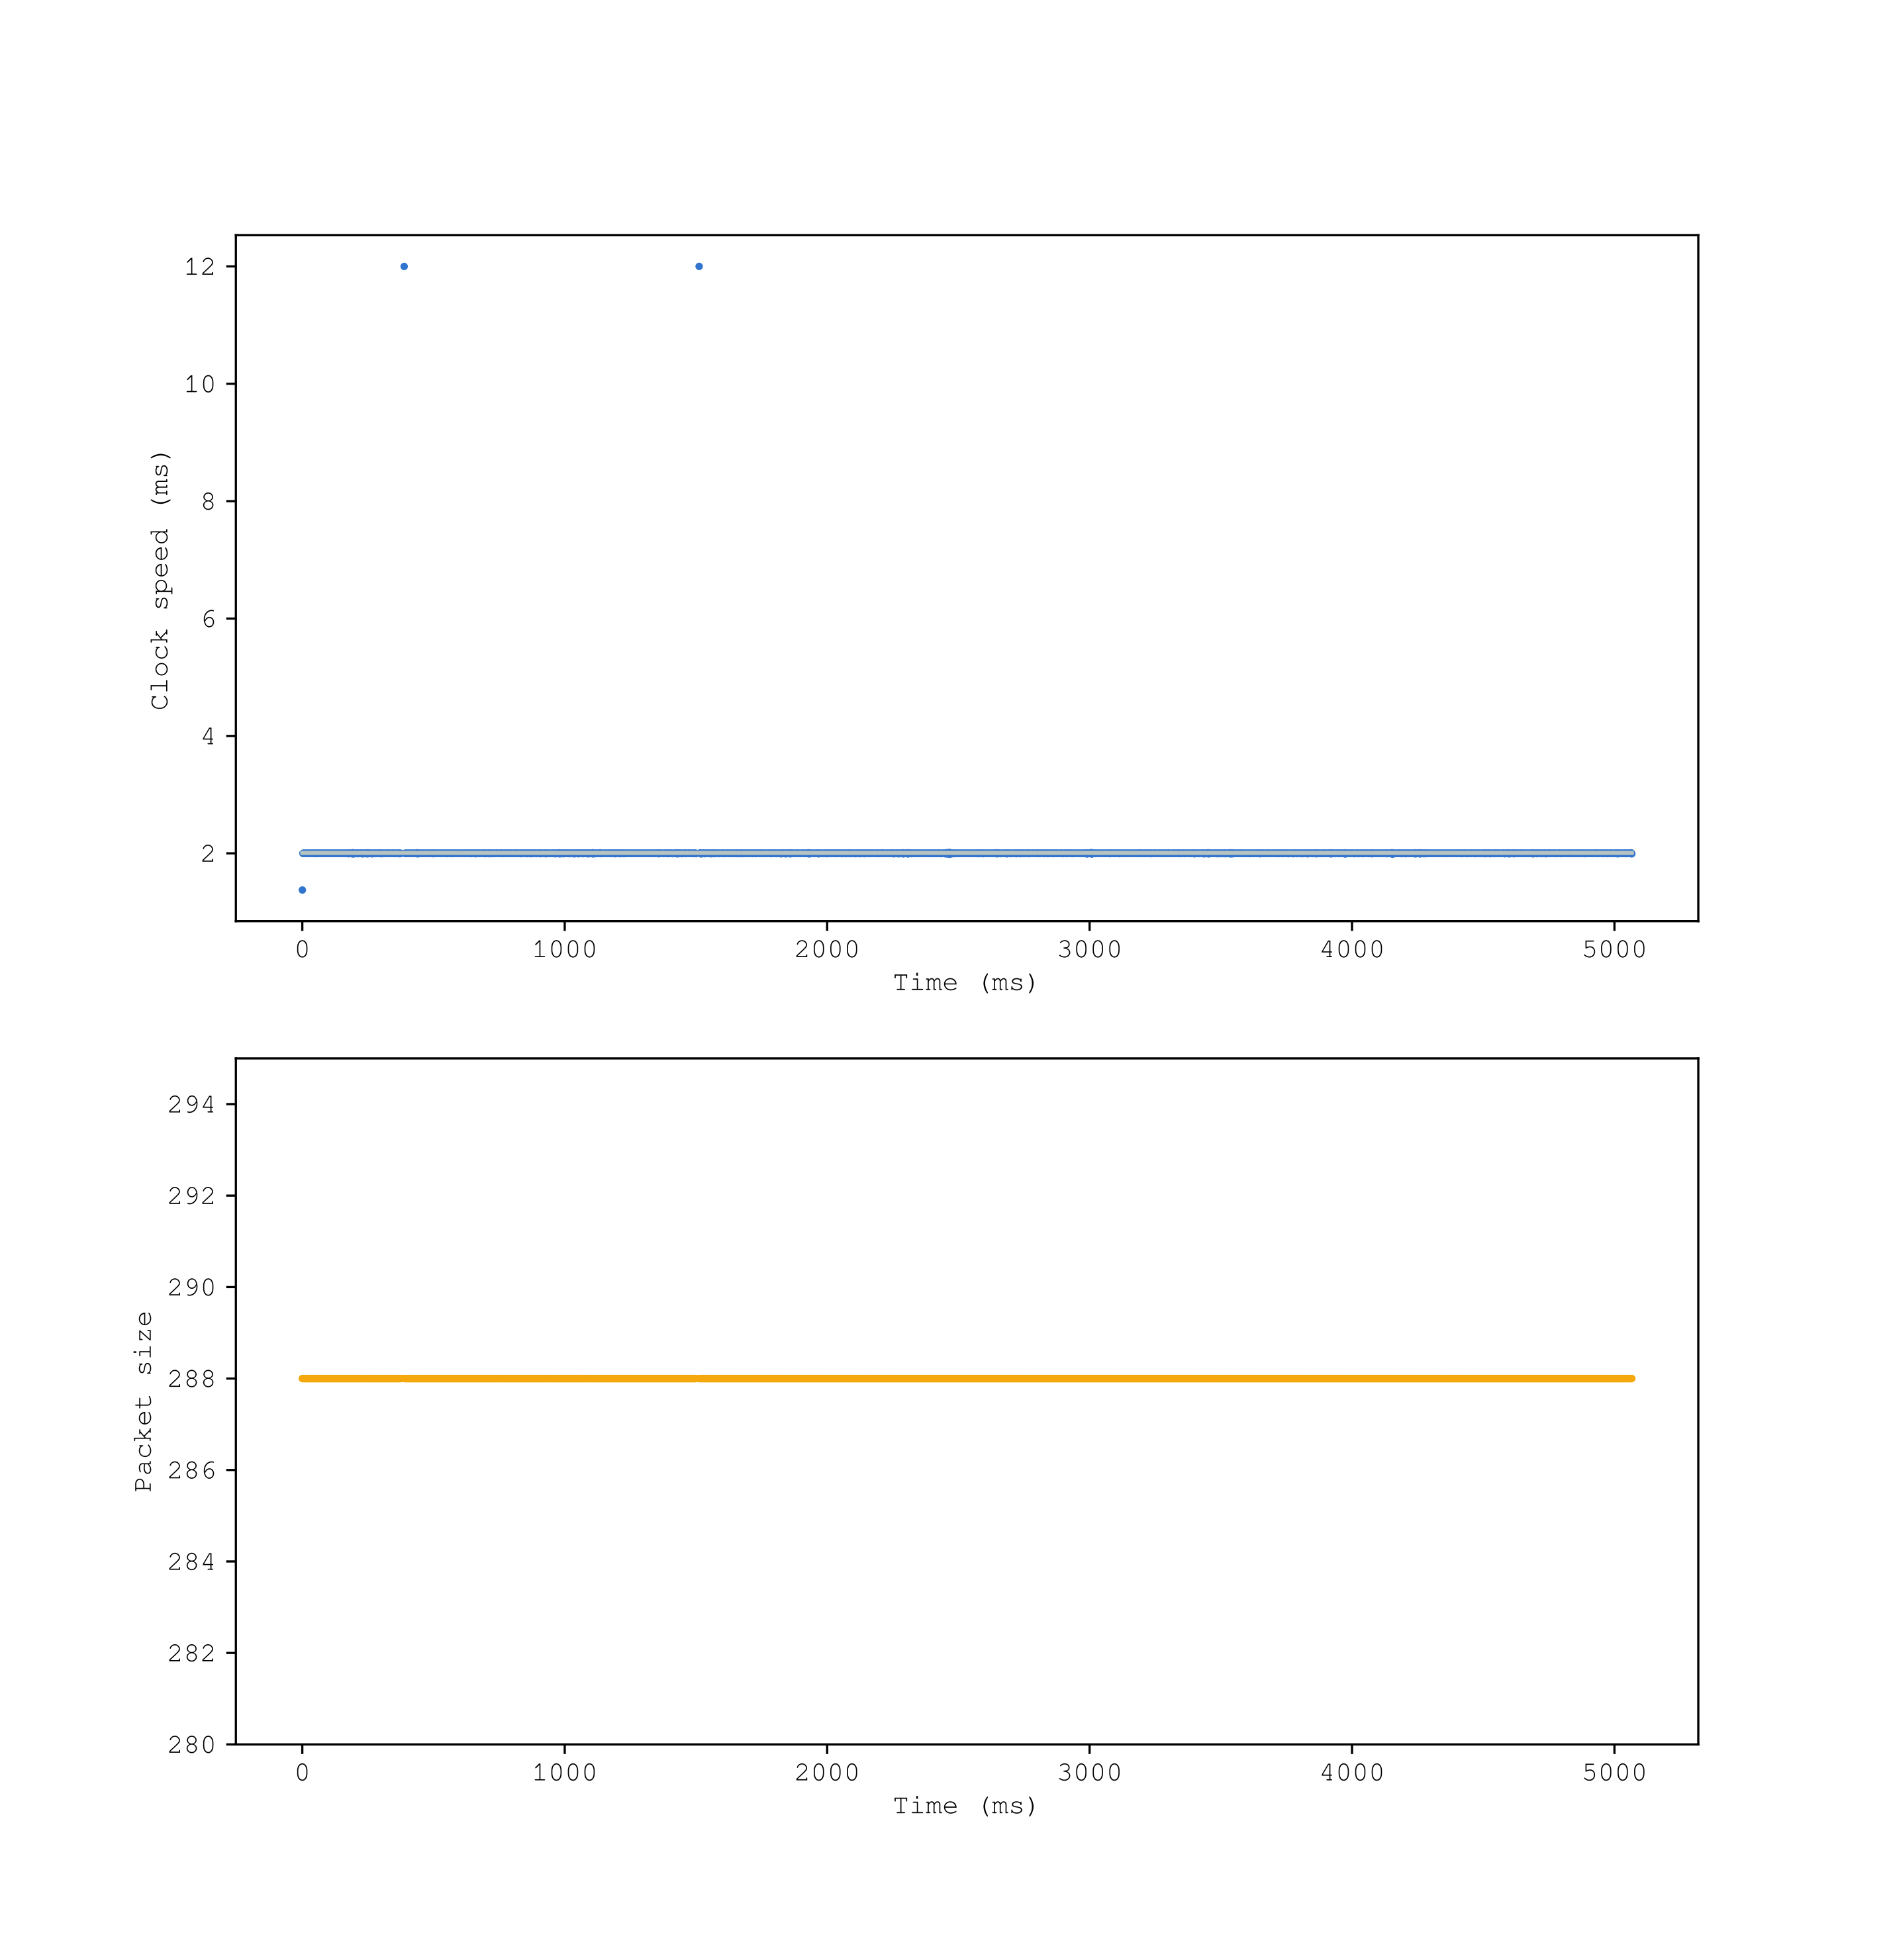
\includegraphics[width=0.8\textwidth]{Experiment-1/Experiment-1-1.png}
	\label{fig:experiment-1-1}
\end{figure}
